\documentclass[12pt, letterpaper, final, onecolumn, titlepage] {article}

\usepackage{enumerate}
\usepackage{graphicx}
\usepackage{listings}
\usepackage{color}
\usepackage{setspace}
\usepackage[margin=1in]{geometry}
\usepackage{mathtools}
\usepackage{amsmath}
\usepackage{hyperref}

\title{ECE 528: Cloud Computing \\
	\vspace{1.5cm}
   		\begin{center}
\includegraphics{umlogo} \end{center}
	\vspace{1.5cm}
	\textbf{Assignment \#5} \\
Midterm Tutorial Execution: Deploying an API with AWS Lambda and AWS API Gateway}
	
\author{Michael Bowyer}

\date{\today}

\definecolor{dkgreen}{rgb}{0,0.6,0}
\definecolor{gray}{rgb}{0.5,0.5,0.5}
\definecolor{mauve}{rgb}{0.58,0,0.82}

\lstset{frame=tb,
  language=C,
  aboveskip=3mm,
  belowskip=3mm,
  showstringspaces=false,
  columns=flexible,
  basicstyle={\small\ttfamily},
  numbers=none,
  numberstyle=\tiny\color{gray},
  keywordstyle=\color{blue},
  commentstyle=\color{dkgreen},
  stringstyle=\color{mauve},
  breaklines=true,
  breakatwhitespace=true,
  tabsize=3
}

\begin{document}

\maketitle

\doublespacing

\section{Assignment Description}

This assignment entails following the prescribed exercise steps created by another student in the ECE 528 course. The excersise steps I have selected for this assignment is that made by Jake Huneau, who describes what steps to take to utilize AWS Lambda and API Gateway for hosting an API.

The steps described in the exercise of his tutorial indicate the following:
\begin{enumerate}
	\item Update your API code so it includes a POST, PUT, and DELETE HTTP method
	\item Upload your code to AWS Lambda using AWS s3 instead of uploading a zip
	\item Set up another AWS Lambda function for a production version of your code
	\item Set up your code pipeline so it automatically uploads changes to your code to AWS Lambda and also updates the dev version of API Gateway
\end{enumerate}

The items themselves are a little confusing, as it appears item number three is redundant of item one. Item one indicates the creation of a new API with mutliple methods, while item three indicates the setup of a new lambda function. Therefore, I have combined items one and three into the creation of a single lamda function which is for a new API I have written. Item two is deploying it using AWS S3 rather than the inline editor which is described in the following sections. Item four, however, is unfortunately vague and lacking details in the tutorial itself, so it isn't clear how to complete this step due to the fact that it appears to rely on other AWS services not described in the tutorial such as AWS CodePipeline. Instead of conducitng this step, proof that the API has been sucessully deployed to AWS API Gateway is provided.

\section{Description of work done}
\subsection{Update your API code so it includes a POST, PUT, and DELETE HTTP method}

The first step I took to accomplishing the excersises was to make my own API which differences from the tutorial so that I could gain knowledge of how to do so. The API I made was a simple sports team finder/editor one. The general idea is that someone can query the API to do the following:
\begin{enumerate}
	\item Get all of the team names in the NFL, NBA, or EPL (GET)
	\item Find if a team exists in any of those leagues (GET)
	\item Find what league a team belongs to (GET)
	\item Add a new team to a league (POST)
	\item Update a team name (PUT)
	\item Delete a team from a league (DELETE)
\end{enumerate}

Each of these API calls are demonstrated in the below images locally using uvicorn and fastapi as described in the tutorial.
\begin{figure}[htbp]
	\centerline{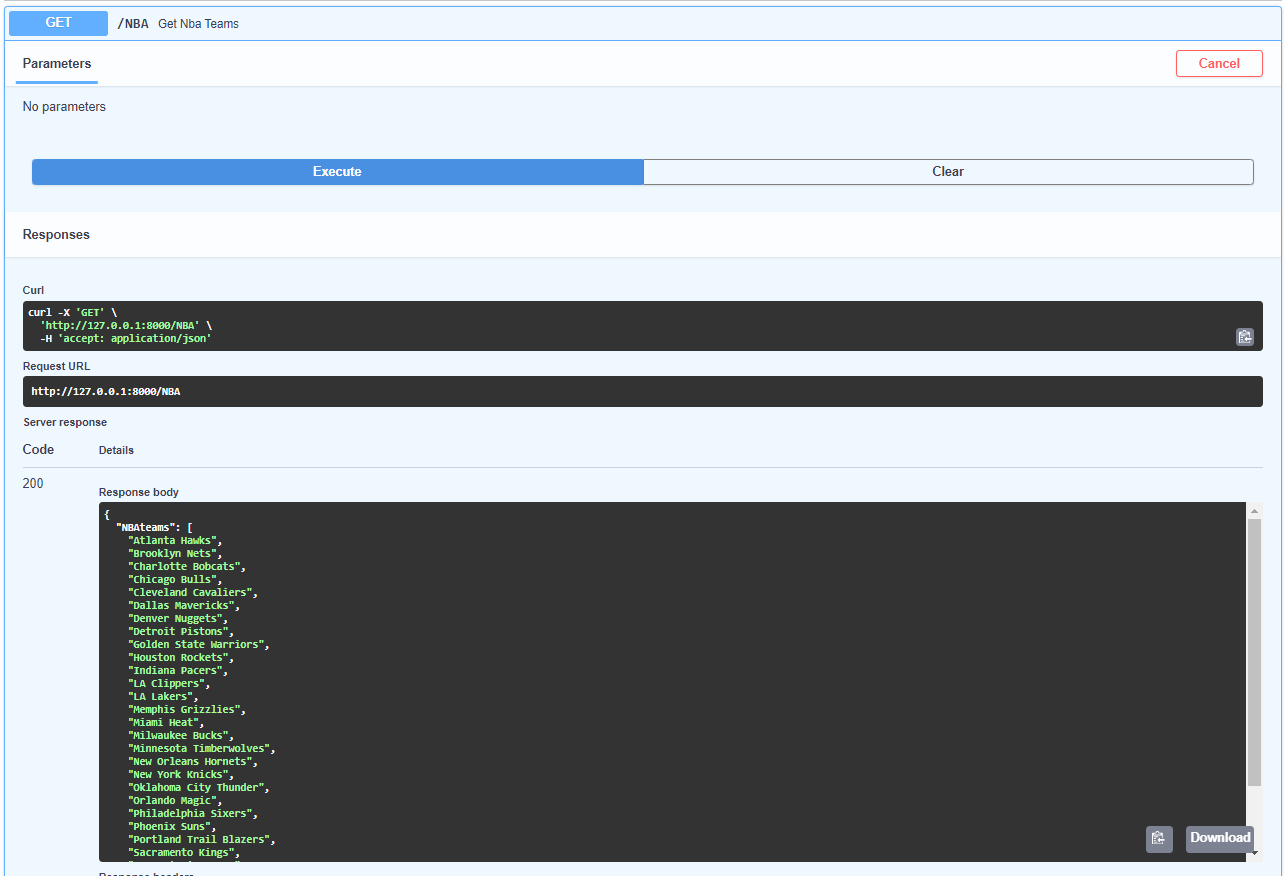
\includegraphics[scale=.4]{4/Get_NBA.png}}
	\caption{GET API function definition for obtaining all NBA team list }
	\label{getNBA}
\end{figure}

\begin{figure}[htbp]
	\centerline{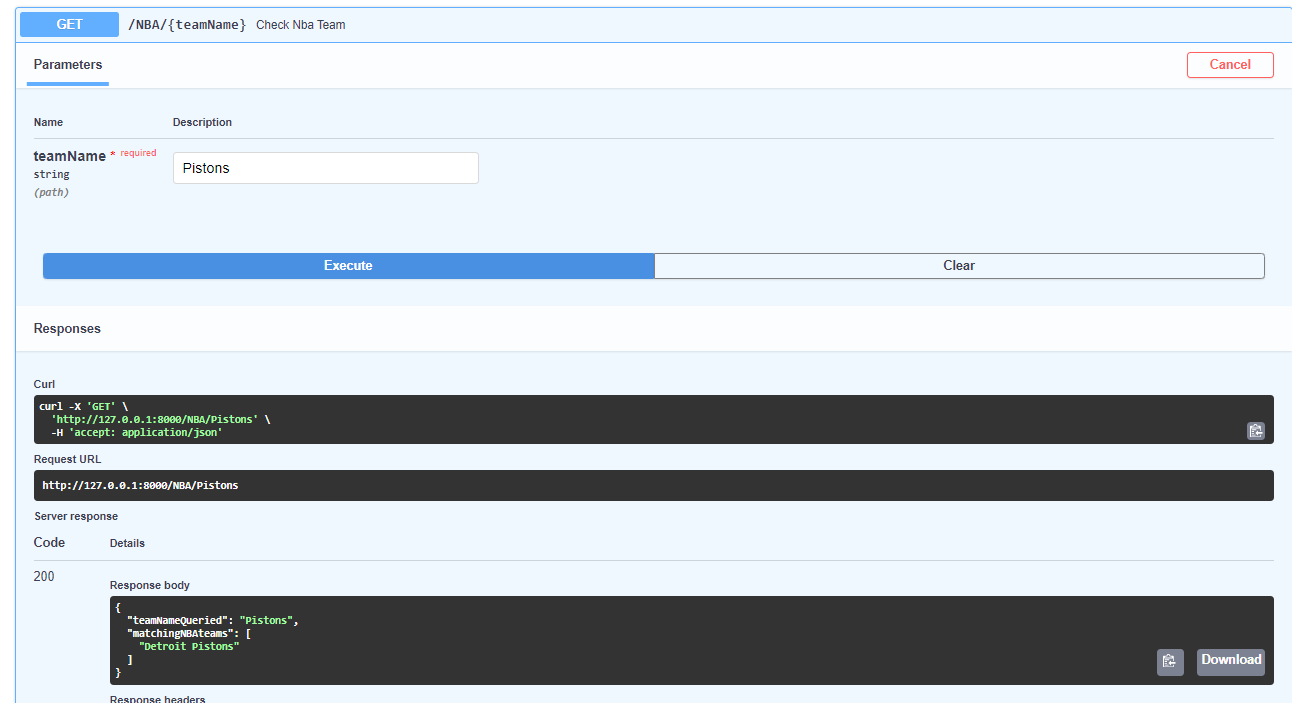
\includegraphics[scale=.4]{4/Get_NBA_team.png}}
	\caption{GET API function definition for getting NBA teams which meets a given name}
	\label{getNBATeam}
\end{figure}

\begin{figure}[htbp]
	\centerline{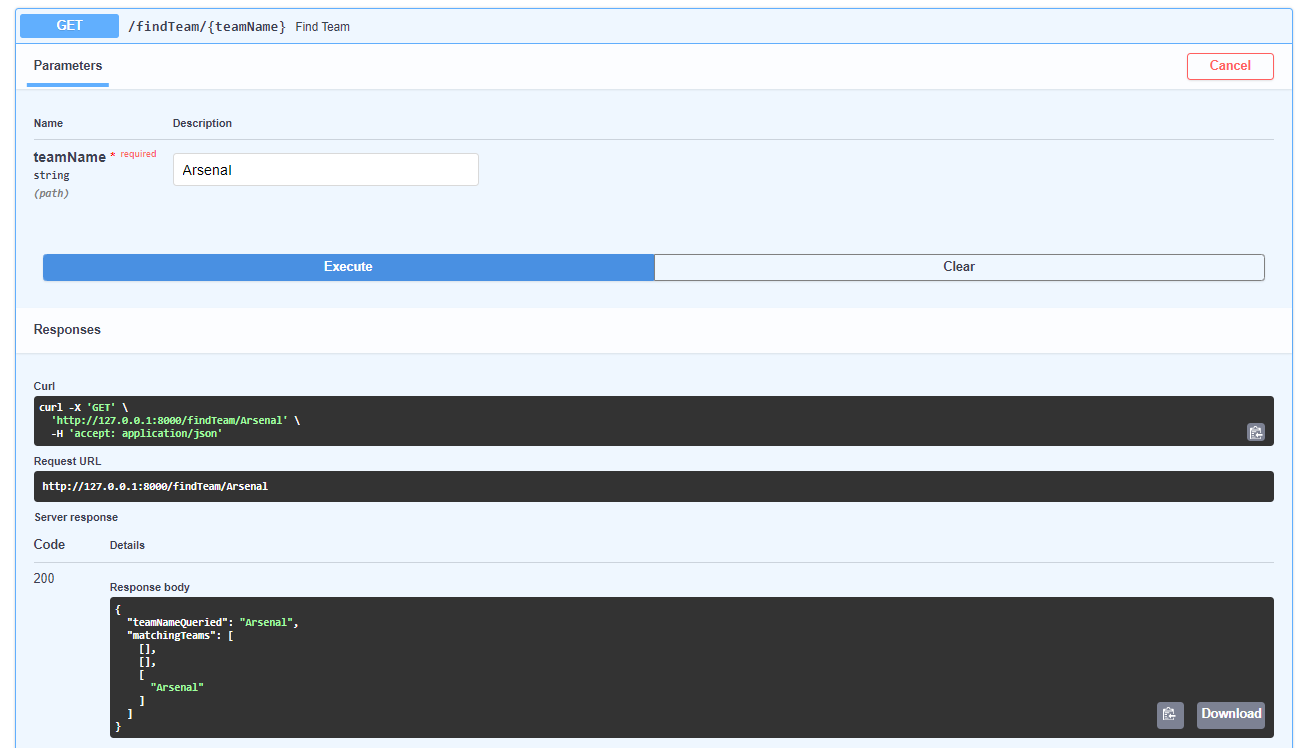
\includegraphics[scale=.4]{4/Get_FindTeam.png}}
	\caption{GET API function definition for finding any team in any league which meets a given name}
	\label{getfindTeam}
\end{figure}

\begin{figure}[htbp]
	\centerline{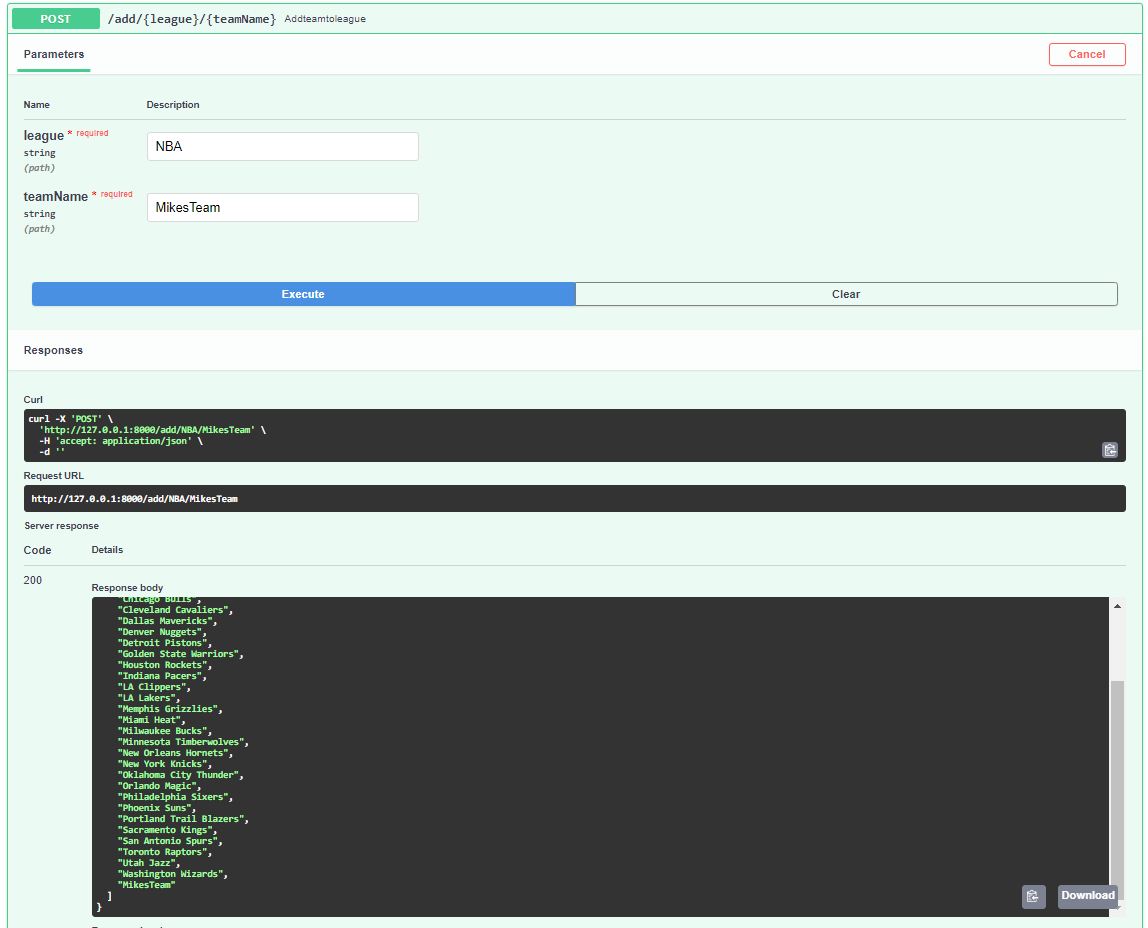
\includegraphics[scale=.4]{4/Post_mikesteam.png}}
	\caption{POST API function definition for adding a new team to a given league}
	\label{postTeam}
\end{figure}

\begin{figure}[htbp]
	\centerline{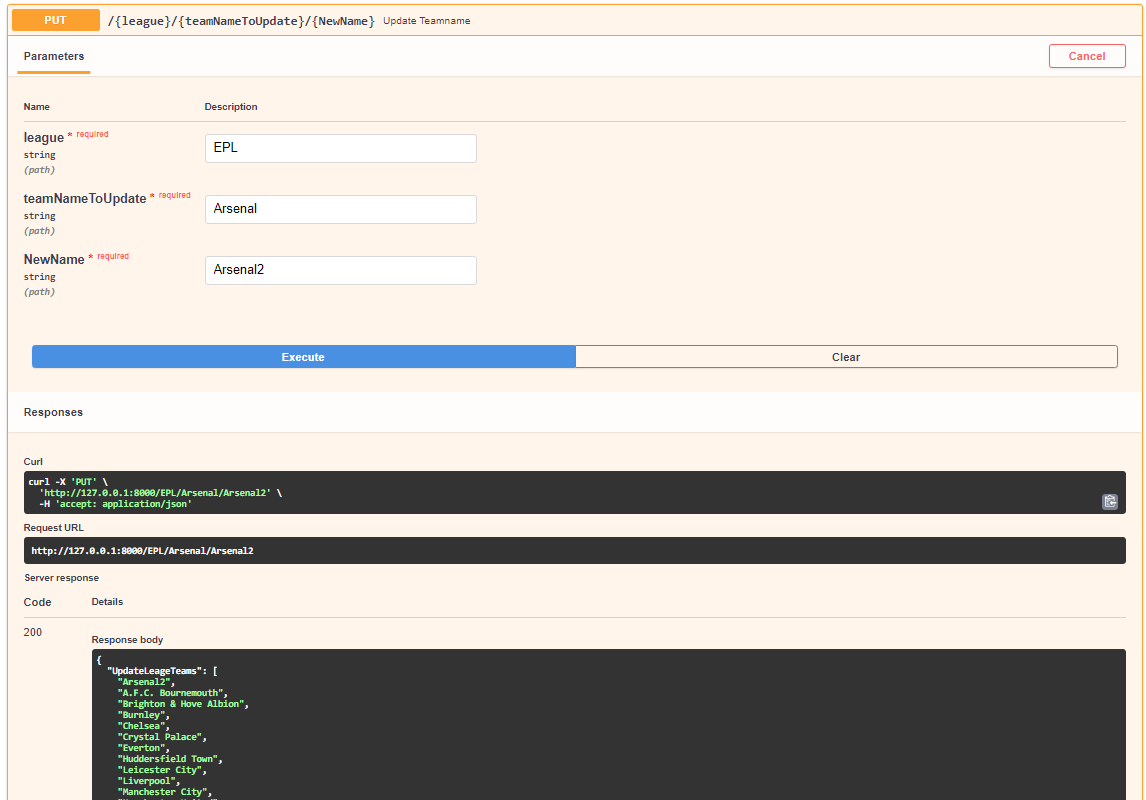
\includegraphics[scale=.4]{4/put_Arsenal2.png}}
	\caption{PUT API function definition for updating a team name in a given league}
	\label{putTeam}
\end{figure}

\begin{figure}[htbp]
	\centerline{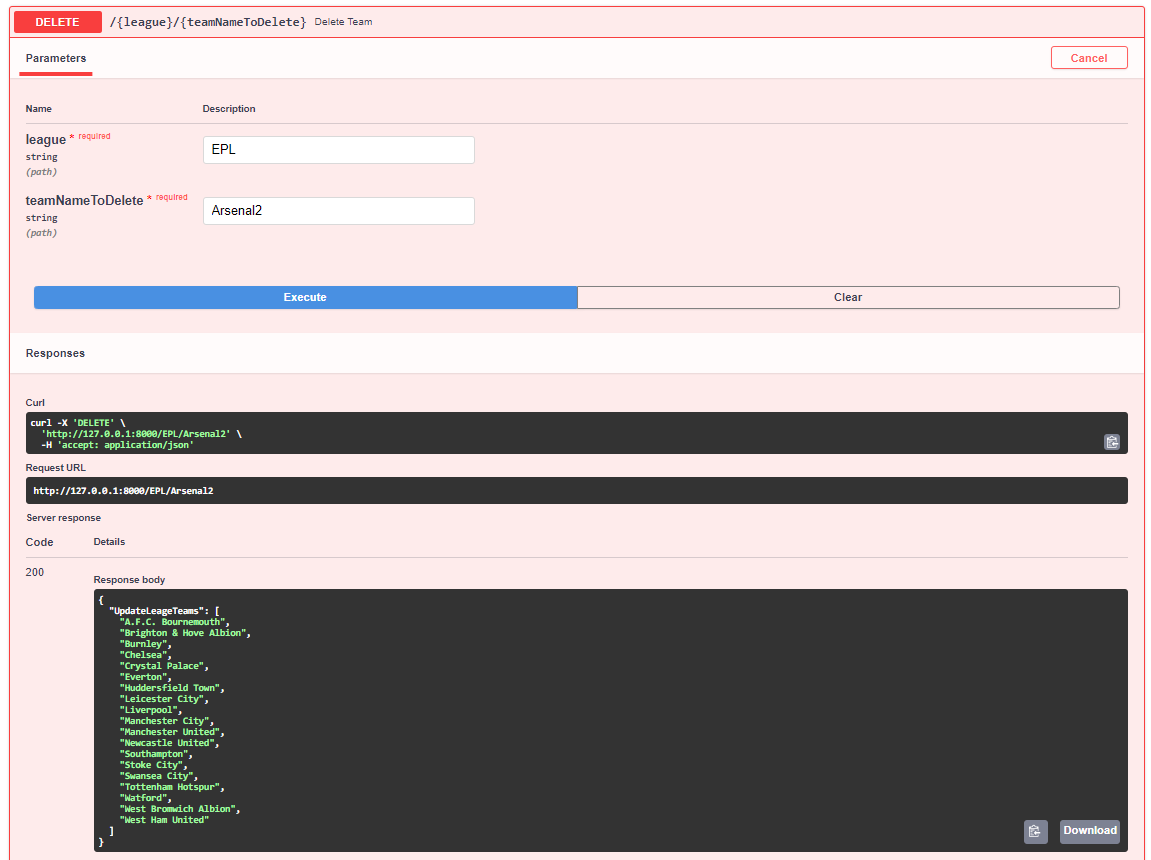
\includegraphics[scale=.4]{4/delete_aresnal2.png}}
	\caption{DELETE API function definition for deleting a team name in a given league}
	\label{deleteTeam}
\end{figure}
\pagebreak

\subsection{Upload your code to AWS Lambda using AWS s3 instead of uploading a zip}
It is a little difficult to prove that an AWS lambda function is actually using a zip file, but the following images are my best attempt to prove that it was completed.

\begin{figure}[htbp]
	\centerline{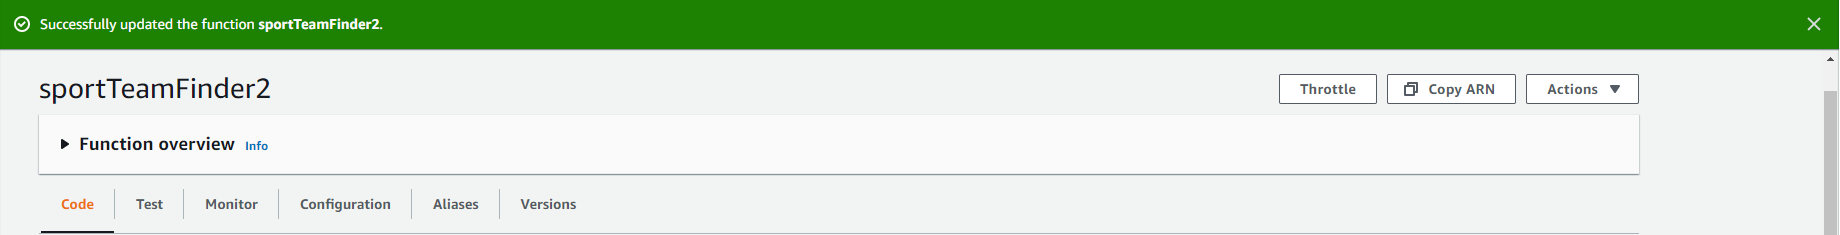
\includegraphics[scale=.4]{1/sucessfulUpdate.png}}
	\caption{Proof of successful update of lambda function after connecting it to S3 storage }
	\label{sucessfulUpdate}
\end{figure}
\begin{figure}[htbp]
	\centerline{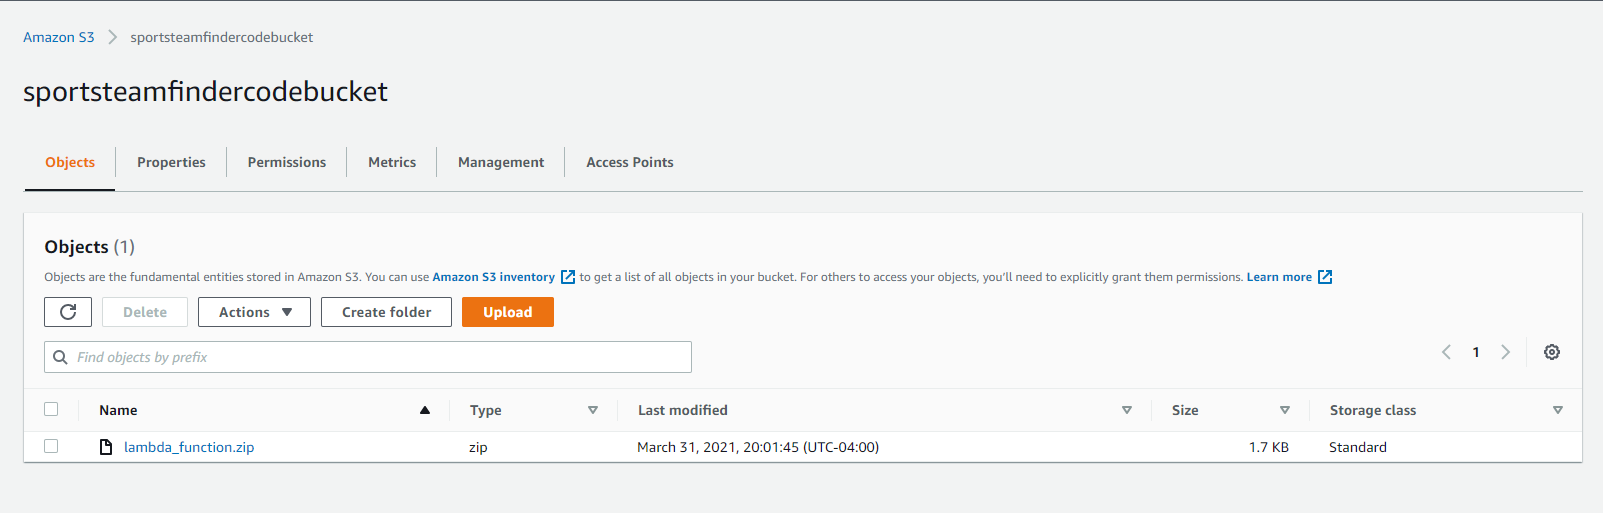
\includegraphics[scale=.4]{1/S3_Proof.png}}
	\caption{Proof of existing S3 bucket containing API code}
	\label{S3Proof}
\end{figure}

\subsection{Connect AWS Lambda Function to API Gateway}
Finally, the API developed was connected to the API Gateway and the GET methods were tested. The below images show the result of the tests.

\begin{figure}[htbp]
	\centerline{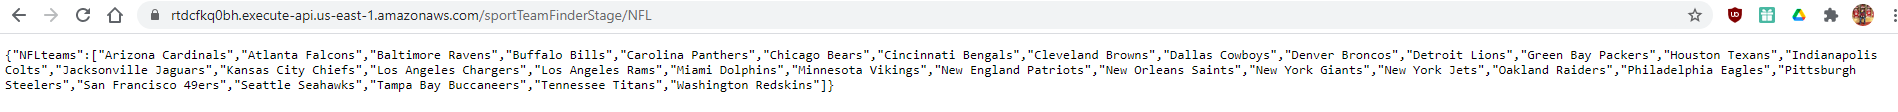
\includegraphics[scale=.4]{3/NFLResult.png}}
	\caption{Proof of NFL GET method returns all NFL teams from AWS API Gateway URL }
	\label{getNFL}
\end{figure}
\begin{figure}[htbp]
	\centerline{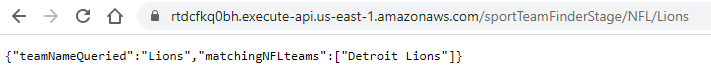
\includegraphics[scale=.4]{3/NFLLions.png}}
	\caption{Proof of NFL GET method returns Detroit Lions when queried for "Lions"}
	\label{getLions}
\end{figure}

\section{Code}

All code generated within scope of this assignment can be found in the Assignment 5 folder in the GitHub repository:
\url{https://github.com/mikebowyer/ECE528_Assignments}.


\end{document}

